\section{Injection Strategy}

The LUX collaboration agreed upon a three phase plan for a safe and successful tritium injection.  The first phase of this plan was a natural methane injection using the tritiated methane injection system for the purpose of determining the purification time constant in LUX.  The second phase of the plan was a small tritium injection (19 mBq) into LUX.  This small injection would highlight any potential problems before injecting a larger amount of tritium, and it would determine if any scaling factor was needed between the absolute injection activity and the observed injection activity.  Additionally, the small tritium injection would allow us to measure the fraction of tritium that goes into the fiducial volume.  Finally, the third phase of the plan was to use what we learned from the first two phases to safely inject a larger amount of tritium (15,000 events) for the purpose of measuring the ER rejection factor of LUX and cross-checking the NEST prediction of the ER band.

NOTE: SHOULD I PUT 19 mBq as the target, or adjust it now that we know the factor of 2 issue? The number of events and the target rate are not what we actually got, but we know this is due to the volume measurements being off.


\subsection{Phase One}

During phase one 0.02 grams of natural methane were injected into LUX using the tritium injection system.  Purity samples from the detector were collected over the next few days, and a purification time constant of 5.90 $\pm$ 0.07 hours was determined using data collected with the LUX gas sampling system.

NOTE: ASK JON FOR EXACT METHANE AMOUNT

\begin{figure}[H]
\centering
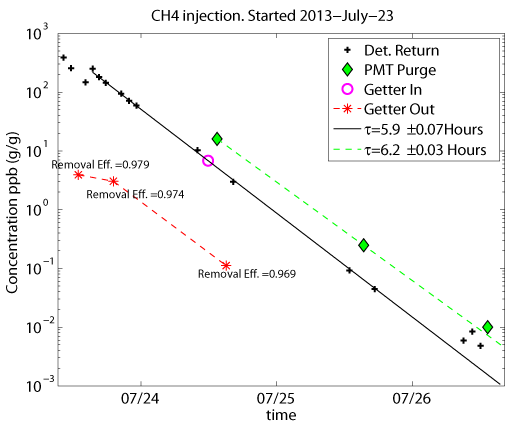
\includegraphics[scale=0.3]{CH4_injection.png}
\caption{First three days of the natural methane injection.  The discontinuity near the beginning of the data is due to a secondary natural methane injection.}
\label{fig:CH4Inject}
\end{figure}

\subsection{Phase Two}

During phase two ?? $\pm$ ?? mBq of CH$_3$T was injected into LUX.  The simulations which are discussed in section ?? predicted that we should see ?? events in the fiducial volume given a ?? mBq injection, a six hour purification time constant, and an immediate removal of 20\% of the injected activity by the purifier.  The immediate removal of 20\% of the injected activity was motivated by what we have seen during the natural methane injection into LUX.  These simulations assumed that the remaining 80\% of the activity would go into the liquid xenon in the detector, and that the fiducial fraction would be $\frac{100}{375}=26.6\%$.


\begin{figure}[H]
\centering
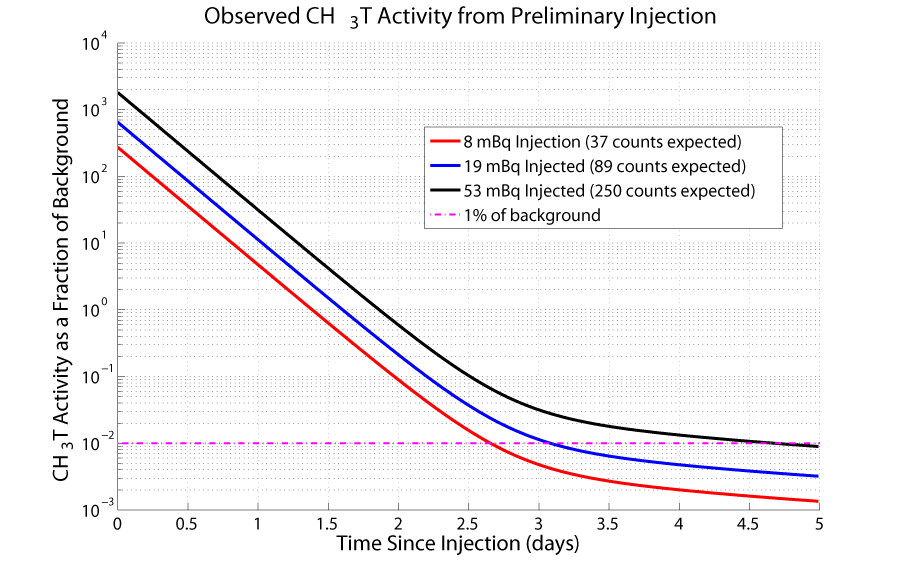
\includegraphics[scale=0.2]{LUX_prelimCH3T.png}
\caption{Simulation of various tritium injections into LUX.}
\label{fig:LUXPrelim}
\end{figure}

The first 23 hours of data show that the initial injection activity in the fiducial volume was 24.2 $\pm$ 0.3 mBq, while the initial injection activity in the entire detector was 44.9 $\pm$ 0.5 mBq.  For this analysis we define the fiducial region as being 30 to 320 $\mu$s in Z = 45cm. (1.55 mm/$\mu$s drift), with r $<$ 17.5 cm. The activity fell with a purification time constant of 6.9 $\pm$ 0.4 hours within the fiducial volume, and a purification time constant of 7.7 $\pm$ 0.4 hours in the entire detector.  

\begin{figure}[H]
\centering
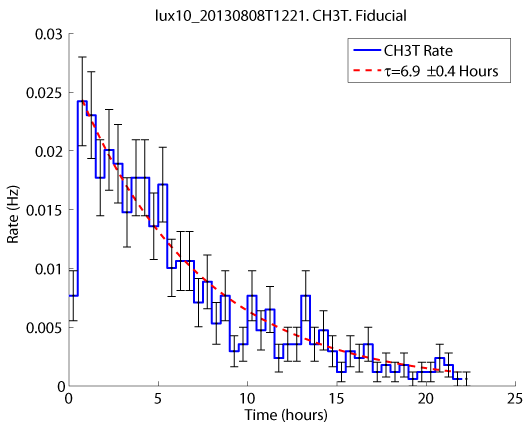
\includegraphics[scale=0.25]{CH3T_fid_rate_new.png}
\caption{Event rate in fiducial region after the smaller tritium injection into LUX.}
\label{fig:FidRate}
\end{figure}

\begin{figure}[H]
\centering
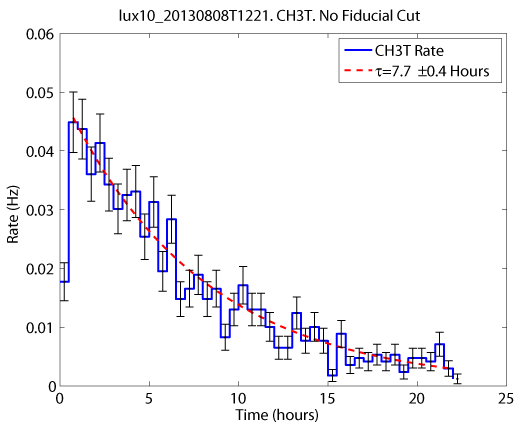
\includegraphics[scale=0.22]{CH3T_no_fid_rate_new.png}
\caption{Event rate in entire detector after the smaller tritium injection into LUX.}
\label{fig:NoFidRate}
\end{figure}


NOTE: UPDATE THESE PLOTS, ESPECIALLY THE SIMULATION PLOT.  CHANGE FIDUCIAL FRACTION IN SIMS TO MATCH DATA ANALYSIS

\subsection{Phase Three}

During phase three ?? $\pm$ ?? mBq was injected into LUX.  The simulations which are discussed in section ?? predicted that we should see ?? events in the fiducial volume given a ?? mBq injection, a six hour purification time constant, and an immediate removal of 20\% of the injected activity by the purifier.  The immediate removal of 20\% of the injected activity was motivated by what we have seen during the natural methane injection into LUX.  These simulations assumed that the remaining 80\% of the activity would go into the liquid xenon in the detector, and that the fiducial fraction would be $\frac{100}{375}=26.6\%$.


NOTE: MAKE PLOT OF SIMULATIONS FOR THIS SET UP

The first ?? hours of data show that the initial injection activity in the fiducial volume was ?? $\pm$ ?? mBq, while the initial injection activity in the entire detector was ?? $\pm$ ?? mBq.  For this analysis we define the fiducial region as being ?? to ?? $\mu$s in Z =  ??cm. (1.55 mm/$\mu$s drift), with r $<$ ?? cm. The activity fell with a purification time constant of ?? $\pm$ ?? hours within the fiducial volume, and a purification time constant of ?? $\pm$ ?? hours in the entire detector.  


NOTE: MAKE PLOTS OF RATES IN FID AND NON FID
